\documentclass[a4paper, 10pt]{article}
%\usepackage{fontspec}
%\setmainfont{Lato}
\usepackage{pgf}
\usepackage{eurosym}
\usepackage{graphicx}
\usepackage{wasysym}
\usepackage{hyperref}
\usepackage{listings}
\usepackage{pxfonts}
\usepackage{verbatim}
\usepackage{color}
\usepackage{xcolor}
\usepackage{wrapfig}
\usepackage{enumitem}
\usepackage{booktabs}
\usepackage{gensymb}
\usepackage{tabularx}
\usepackage{currfile}

\hypersetup{
    bookmarks=true,         % show bookmarks bar?
    unicode=true,          % non-Latin characters in Acrobat’s bookmarks
    pdftoolbar=true,        % show Acrobat’s toolbar?
    pdfmenubar=true,        % show Acrobat’s menu?
    pdffitwindow=true,     % window fit to page when opened
    pdftitle={Assessments},    % title
    pdfauthor={Paul Vesey},     % author
    pdfsubject={Advanced Graphics Assignment },   % subject of the document
    pdfcreator={},   % creator of the document
    pdfproducer={xelatex}, % producer of the document
    pdfkeywords={'Graphics' }, % list of keywords
    pdfnewwindow=true,      % links in new PDF window
    colorlinks=true,       % false: boxed links; true: colored links
    linkcolor=violet,          % color of internal links (change box color with linkbordercolor)
    citecolor=magenta,        % color of links to bibliography
    filecolor=red,      % color of file links
    urlcolor=blue           % color of external links
}

\setlength\parindent{0pt}
\begin{document}

\lstset{language=HTML,
				basicstyle=\small,
				breaklines=true,
        numbers=left,
        numberstyle=\tiny,
        showstringspaces=false,
        aboveskip=-20pt,
        frame=leftline
        }
				
\begin{table}%
	\begin{minipage}{0.4\textwidth}%
			
\includegraphics[width=1\textwidth]{./img/LITlogo.jpg}
	\end{minipage}
	\qquad
	\centering
	\parbox{0.4\textwidth}{
		\begin{large}			
			\begin{tabular}{| r | l |} \hline
				Subject: & \textbf{Advanced Graphics}\\
								 & \textbf{\& Visualisation}\\
				Course: & \textbf{Interior Design Y3}\\
				Session: & \textbf{Autumn 2020}\\
				Lecturer: & \textbf{Paul Vesey \footnotesize{BEng, MIE, HDip}}\\
				Filename: & \footnotesize{\currfilename}\\
				\hline
			\end{tabular}
		\end{large}			
	}
\end{table}
\vspace{0.25cm}	
	
\begin{flushleft}
\Large\textbf{Photography Trip - Limerick }\\
\end{flushleft}

The objective of this exercise is to explore and develop your image creation abilities.  This will be achieved by capturing 10 images using your own camera or camera-phone, based on an allocated theme.  The themes will be allocated by random selection at the beginning of the session.\\

For this exercise you will work in pairs.  Please note that you will be taking images in public areas.  You should avoid taking images of people.  Also please note that you must act responsibly and safely at all times.\\

Your images must be consistent with the theme provided. Your images will be judged on how well they fit the theme; framing; composition, etc. Take your
time when setting up, and creating these images; ensure there is a sequence and story to them.\\

Try to avoid ’documentary’ images and eye level images.\\

In the following class session, each pair will present their images on a power-point presentation for critique by the class members.\\

The themes are as follows:

\begin{enumerate}
	\item Old \& New in Harmony
	\item City Life
	\item Visual Noise
	\item Pattern and Texture
	\item Clash - who let this happen?
	\item Cultural Diversity
	\item The Wall
	\item Inhabitants of the Empty
	\item Instant Gratification
	\item A splash of color in a grey world
\end{enumerate}

For this exercise we will meet at 2:00pm at the corner of O'Connell Street and Cruise's Street, where themes will be allocated.\\

In addition to image creation, you will purchase an item in a charity shop for reproduction in 3D Studio.  There are a number of charity shops in Limerick in the Thomas Street area.  \textbf{We will regroup at 4:00pm at the SVP shop in Thomas Street where you can select an item for purchase}. Please note that I will approve the suitability of the item you intend to model.\\

\begin{figure}[ht]
	\centering
		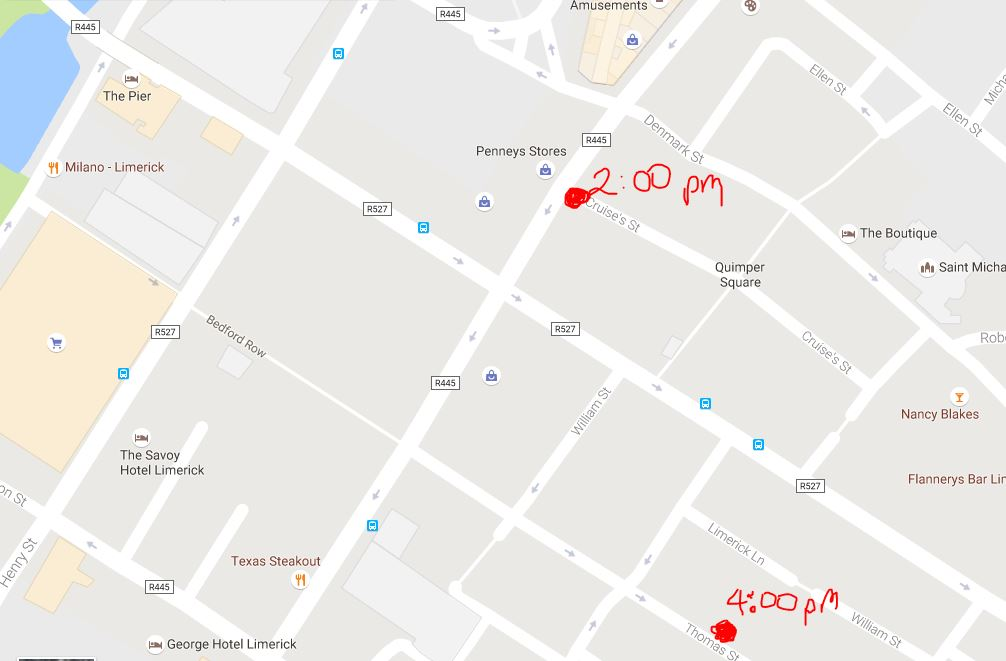
\includegraphics[width=12cm]{img/LKMap.JPG}
	\caption{Meeting Locations}
	\label{fig:LKMap}
\end{figure}



\begin{figure}[ht]
	\centering
		\includegraphics[width=10cm]{img/LK1.JPG}
	\caption{Sample Image 1}
	\label{fig:LK1}
\end{figure}


\begin{figure}[ht]
	\centering
		\includegraphics[width=10cm]{img/LK2.JPG}
	\caption{Sample Image 2}
	\label{fig:LK2}
\end{figure}


\begin{figure}[ht]
	\centering
		\includegraphics[width=10cm]{img/LK3.JPG}
	\caption{Sample Image 3}
	\label{fig:LK3}
\end{figure}

\begin{figure}[ht]
	\centering
		\includegraphics[width=10cm]{img/LK4.JPG}
	\caption{Sample Image 4}
	\label{fig:LK4}
\end{figure}




\end{document}